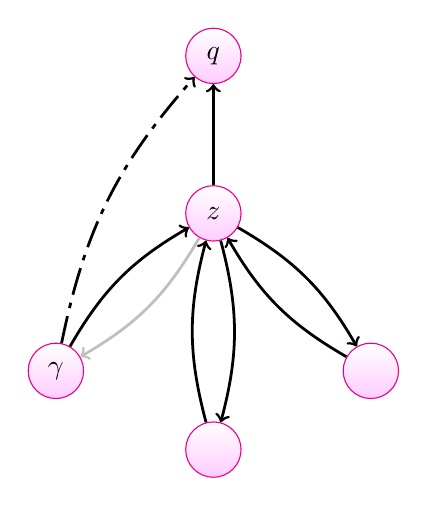
\begin{tikzpicture}

\tikzset{mynode2/.style={circle,minimum size=20pt,inner sep=0pt,draw, top color=white ,bottom color=magenta!20, magenta,text=black},}
\tikzset{mynode7/.style={circle,fill=gray,minimum size=20pt,inner sep=0pt,},draw}


  \draw (0,1) node[mynode2](gamma) {$\gamma$};
  \draw (2,0) node[mynode2] (n1){};  
  \draw (4,1) node[mynode2](n2) {};
  \draw (2, 3) node[mynode2](z) {$z$}; 
  \draw (2,5) node[mynode2](q) {$q$};
              
              
  %edges for z
    \draw[->, line width=1pt] (n1) to[bend left=15](z);
    \draw[->, line width=1pt] (n2)to[bend left=15] (z);
	\draw[->, line width=1pt] (gamma)to[bend left=15] (z);    
    
    \draw[->,line width=1pt] (z) to[bend left=15](n1);
    \draw[->,line width=1pt] (z)to[bend left=15] (n2);
    
     \draw[->,line width=1pt] (z) --(q);
    \draw[->,gray!50,line width=1pt] (z)to[bend left=15] (gamma); 
     \draw[->, dash pattern=on 10pt off 3pt on 2pt off 3pt , line width=1pt] (gamma)to[bend left=15] (q);   
    
\end{tikzpicture}
